\chapter{Layout Algorithms}
\label{chap:layout-algorithms}

When loading a Petri net without position information, or after extensive manual editing, the diagram can become cluttered and difficult to read. This chapter covers the automatic layout algorithms that transform messy diagrams into clear, structured visualizations.

\section{Problem Statement}
\label{sec:layout-problem}

Consider importing a PNML file from another tool that stored no graphical information. All elements would be placed at position $(0, 0)$, creating an unusable overlap. Even with positions, diagrams can suffer from:

\begin{itemize}
    \item \textbf{Overlapping elements}: Places and transitions stacked on each other
    \item \textbf{Arc crossings}: Lines crossing unnecessarily, obscuring the flow
    \item \textbf{Poor spacing}: Elements too close or too far apart
    \item \textbf{No visual hierarchy}: The logical flow of the process is not apparent
\end{itemize}

Layout algorithms solve these problems by calculating optimal positions for all elements.

\section{Available Algorithms}
\label{sec:layout-algorithms}

The application provides two layout algorithms with different characteristics:

\begin{table}[htb]
    \centering
    \begin{tabular}{lll}
        \toprule
        \textbf{Algorithm} & \textbf{Approach} & \textbf{Best For} \\
        \midrule
        Spring Embedder & Physics simulation & General, organic layouts \\
        Sugiyama & Hierarchical layering & Sequential processes, flowcharts \\
        \bottomrule
    \end{tabular}
    \caption{Layout algorithm comparison}
    \label{tab:layout-comparison}
\end{table}

\section{Spring Embedder Algorithm}
\label{sec:spring-embedder}

The Spring Embedder models the Petri net as a physical system:

\begin{itemize}
    \item \textbf{Nodes} act as electrically charged particles that \textbf{repel} each other
    \item \textbf{Arcs} act as springs that \textbf{attract} connected nodes toward an ideal length
\end{itemize}

The algorithm iteratively moves nodes until forces reach equilibrium.

\subsection{Force Calculation}

For each node, the total force is the sum of:
\begin{enumerate}
    \item \textbf{Repulsion} from all other nodes: $F_{rep} = \frac{C_{rep}}{d^2}$
    \item \textbf{Spring attraction/repulsion} from connected nodes: $F_{spring} = C_{spring} \cdot (d - L)$
\end{enumerate}

Where $d$ is the distance between nodes, $L$ is the ideal arc length, and $C_{rep}$, $C_{spring}$ are constants.

\begin{lstlisting}[language=TypeScript, caption={Spring Embedder implementation (src/app/tr-services/layout-spring-embedder.service.ts)}]
import { Injectable } from '@angular/core';
import { DataService } from './data.service';
import { Point } from '../tr-classes/petri-net/point';
import { Node } from '../tr-interfaces/petri-net/node';

@Injectable({ providedIn: 'root' })
export class LayoutSpringEmbedderService {
    // Algorithm parameters
    private epsilon = 0.01;       // Minimum force for termination
    private maxIterations = 5000; // Maximum iteration count
    private cRep = 20000;         // Repulsion constant
    private idealLength = 150;    // Ideal arc length
    private cSpring = 20;         // Spring constant

    constructor(private dataService: DataService) {}

    /**
     * Apply Spring Embedder layout to all nodes.
     * Runs asynchronously with visual feedback.
     */
    async layoutSpringEmbedder(): Promise<void> {
        const nodes: Node[] = [
            ...this.dataService.getPlaces(),
            ...this.dataService.getTransitions()
        ];

        // Initialize random positions if all at origin
        this.initializePositions(nodes);

        let maxForce = this.epsilon + 1;
        let iteration = 0;

        // Iterate until equilibrium or max iterations
        while (iteration < this.maxIterations && maxForce > this.epsilon) {
            const forces: Map<string, Point> = new Map();

            // Calculate forces for each node
            for (const node of nodes) {
                const force = this.calculateTotalForce(node, nodes);
                forces.set(node.id, force);
            }

            // Apply forces and track maximum
            maxForce = 0;
            for (const node of nodes) {
                const force = forces.get(node.id)!;
                node.position.x += force.x;
                node.position.y += force.y;

                const magnitude = Math.sqrt(force.x ** 2 + force.y ** 2);
                maxForce = Math.max(maxForce, magnitude);
            }

            // Yield for UI updates (every 10 iterations)
            if (iteration % 10 === 0) {
                this.dataService.triggerDataChanged();
                await this.sleep(1);
            }

            iteration++;
        }

        console.log(`Spring Embedder completed in ${iteration} iterations`);
        this.dataService.triggerDataChanged(true);
    }

    /**
     * Calculate total force on a node from all other nodes.
     */
    private calculateTotalForce(node: Node, allNodes: Node[]): Point {
        let fx = 0, fy = 0;

        for (const other of allNodes) {
            if (other.id === node.id) continue;

            // Repulsion force (always present)
            const repulsion = this.calculateRepulsion(node.position, other.position);
            fx += repulsion.x;
            fy += repulsion.y;

            // Spring force (only for connected nodes)
            if (this.areConnected(node, other)) {
                const spring = this.calculateSpring(node.position, other.position);
                fx += spring.x;
                fy += spring.y;
            }
        }

        return new Point(fx, fy);
    }

    /**
     * Calculate repulsion force between two positions.
     * Inversely proportional to distance squared.
     */
    private calculateRepulsion(p1: Point, p2: Point): Point {
        const dx = p1.x - p2.x;
        const dy = p1.y - p2.y;
        const distance = Math.sqrt(dx * dx + dy * dy);

        // Prevent division by zero
        if (distance < 0.1) {
            return new Point(
                (Math.random() - 0.5) * 10,
                (Math.random() - 0.5) * 10
            );
        }

        const factor = this.cRep / (distance * distance);
        return new Point(
            (dx / distance) * factor,
            (dy / distance) * factor
        );
    }

    /**
     * Calculate spring force between connected nodes.
     * Attracts if too far, repels if too close.
     */
    private calculateSpring(p1: Point, p2: Point): Point {
        const dx = p2.x - p1.x;
        const dy = p2.y - p1.y;
        const distance = Math.sqrt(dx * dx + dy * dy);

        if (distance < 0.1) return new Point(0, 0);

        // Displacement from ideal length
        const displacement = distance - this.idealLength;
        const factor = this.cSpring * displacement / distance;

        return new Point(dx * factor, dy * factor);
    }

    private sleep(ms: number): Promise<void> {
        return new Promise(resolve => setTimeout(resolve, ms));
    }

    // ... helper methods ...
}
\end{lstlisting}

\section{Sugiyama Algorithm}
\label{sec:sugiyama}

The Sugiyama algorithm~\cite{Sugiyama1981} creates hierarchical, layered layouts ideal for sequential processes. It operates in four phases:

\begin{enumerate}
    \item \textbf{Cycle Removal}: Temporarily reverse some arcs to create a DAG
    \item \textbf{Layer Assignment}: Assign nodes to horizontal layers
    \item \textbf{Vertex Ordering}: Order nodes within layers to minimize crossings
    \item \textbf{Coordinate Assignment}: Calculate final x, y positions
\end{enumerate}

\subsection{Phase 1: Cycle Removal}

Petri nets often contain cycles (feedback loops). For hierarchical layout, cycles must be temporarily broken:

\begin{lstlisting}[language=TypeScript, caption={Cycle removal service}]
export class CycleRemovalService {
    private reversedArcs: Arc[] = [];

    constructor(private nodes: Node[], private arcs: Arc[]) {}

    /**
     * Remove cycles by reversing back-edges.
     * Uses depth-first search to detect cycles.
     */
    removeCycles(): void {
        const visited = new Set<string>();
        const recursionStack = new Set<string>();

        for (const node of this.nodes) {
            if (!visited.has(node.id)) {
                this.dfs(node, visited, recursionStack);
            }
        }
    }

    private dfs(node: Node, visited: Set<string>, stack: Set<string>): void {
        visited.add(node.id);
        stack.add(node.id);

        const outgoingArcs = this.arcs.filter(a => a.from.id === node.id);
        
        for (const arc of outgoingArcs) {
            const targetId = arc.to.id;
            
            if (stack.has(targetId)) {
                // Back-edge detected: reverse this arc
                this.reverseArc(arc);
                this.reversedArcs.push(arc);
            } else if (!visited.has(targetId)) {
                this.dfs(arc.to, visited, stack);
            }
        }

        stack.delete(node.id);
    }

    /**
     * Restore reversed arcs after layout is complete.
     */
    reverseArcs(): void {
        for (const arc of this.reversedArcs) {
            this.reverseArc(arc);
        }
    }

    private reverseArc(arc: Arc): void {
        const temp = arc.from;
        arc.from = arc.to;
        arc.to = temp;
    }
}
\end{lstlisting}

\subsection{Phase 2: Layer Assignment}

Nodes are assigned to layers based on their distance from source nodes:

\begin{lstlisting}[language=TypeScript, caption={Layer assignment service}]
export class LayerAssignmentService {
    constructor(private nodes: Node[], private arcs: Arc[]) {}

    /**
     * Assign each node to a layer using longest-path algorithm.
     * Returns array of layers, each containing nodes at that level.
     */
    assignLayers(): Node[][] {
        const layers: Node[][] = [];
        const nodeLayer = new Map<string, number>();

        // Find source nodes (no incoming arcs)
        const sources = this.nodes.filter(n => 
            !this.arcs.some(a => a.to.id === n.id)
        );

        // Assign sources to layer 0
        for (const source of sources) {
            nodeLayer.set(source.id, 0);
        }

        // BFS to assign remaining nodes
        const queue = [...sources];
        while (queue.length > 0) {
            const node = queue.shift()!;
            const currentLayer = nodeLayer.get(node.id)!;

            // Find successors
            const outArcs = this.arcs.filter(a => a.from.id === node.id);
            for (const arc of outArcs) {
                const successor = arc.to;
                const newLayer = currentLayer + 1;

                // Update if this path is longer
                if (!nodeLayer.has(successor.id) || 
                    nodeLayer.get(successor.id)! < newLayer) {
                    nodeLayer.set(successor.id, newLayer);
                    queue.push(successor);
                }
            }
        }

        // Build layer arrays
        const maxLayer = Math.max(...nodeLayer.values());
        for (let i = 0; i <= maxLayer; i++) {
            layers[i] = this.nodes.filter(n => nodeLayer.get(n.id) === i);
        }

        return layers;
    }
}
\end{lstlisting}

\subsection{Phase 3: Vertex Ordering}

Within each layer, nodes are reordered to minimize arc crossings:

\begin{lstlisting}[language=TypeScript, caption={Vertex ordering (barycenter method)}]
export class VertexOrderingService {
    constructor(
        private layers: Node[][],
        private arcs: Arc[]
    ) {}

    /**
     * Order vertices using barycenter heuristic.
     * Minimizes edge crossings between adjacent layers.
     */
    orderVertices(): void {
        // Multiple passes for better results
        for (let pass = 0; pass < 4; pass++) {
            // Forward pass
            for (let i = 1; i < this.layers.length; i++) {
                this.orderLayer(i, i - 1);
            }
            // Backward pass
            for (let i = this.layers.length - 2; i >= 0; i--) {
                this.orderLayer(i, i + 1);
            }
        }
    }

    /**
     * Order nodes in targetLayer based on connections to fixedLayer.
     */
    private orderLayer(targetIdx: number, fixedIdx: number): void {
        const targetLayer = this.layers[targetIdx];
        const fixedLayer = this.layers[fixedIdx];

        // Calculate barycenter for each node
        const barycenters = targetLayer.map(node => {
            const connectedIndices = this.getConnectedIndices(node, fixedLayer);
            if (connectedIndices.length === 0) return Infinity;
            
            const sum = connectedIndices.reduce((a, b) => a + b, 0);
            return sum / connectedIndices.length;
        });

        // Sort by barycenter
        const indexed = targetLayer.map((node, i) => ({ node, bc: barycenters[i] }));
        indexed.sort((a, b) => a.bc - b.bc);
        
        this.layers[targetIdx] = indexed.map(item => item.node);
    }

    private getConnectedIndices(node: Node, layer: Node[]): number[] {
        const indices: number[] = [];
        
        for (const arc of this.arcs) {
            let connected: Node | null = null;
            if (arc.from.id === node.id) connected = arc.to;
            if (arc.to.id === node.id) connected = arc.from;
            
            if (connected) {
                const idx = layer.findIndex(n => n.id === connected!.id);
                if (idx !== -1) indices.push(idx);
            }
        }
        
        return indices;
    }
}
\end{lstlisting}

\subsection{Phase 4: Coordinate Assignment}

Finally, x and y coordinates are calculated based on layers and ordering:

\begin{lstlisting}[language=TypeScript, caption={Coordinate assignment}]
export class CoordinateAssignmentService {
    private layerSpacing = 180;  // Horizontal space between layers
    private nodeSpacing = 100;   // Vertical space between nodes

    constructor(
        private layers: Node[][],
        private canvasWidth: number = 1200,
        private canvasHeight: number = 600
    ) {}

    /**
     * Assign final coordinates to all nodes.
     */
    assignCoordinates(): void {
        const totalWidth = (this.layers.length - 1) * this.layerSpacing;
        const startX = (this.canvasWidth - totalWidth) / 2;

        for (let layerIdx = 0; layerIdx < this.layers.length; layerIdx++) {
            const layer = this.layers[layerIdx];
            const x = startX + layerIdx * this.layerSpacing;

            // Center nodes vertically
            const totalHeight = (layer.length - 1) * this.nodeSpacing;
            const startY = (this.canvasHeight - totalHeight) / 2;

            for (let nodeIdx = 0; nodeIdx < layer.length; nodeIdx++) {
                const node = layer[nodeIdx];
                const y = startY + nodeIdx * this.nodeSpacing;
                
                node.position = new Point(x, y);
            }
        }
    }
}
\end{lstlisting}

\subsection{Orchestrating the Phases}

\begin{lstlisting}[language=TypeScript, caption={Sugiyama layout service (src/app/tr-services/layout-sugiyama.service.ts)}]
@Injectable({ providedIn: 'root' })
export class LayoutSugiyamaService {
    constructor(private dataService: DataService) {}

    /**
     * Apply complete Sugiyama layout algorithm.
     */
    applySugiyamaLayout(): void {
        const nodes = [
            ...this.dataService.getPlaces(),
            ...this.dataService.getTransitions()
        ];
        const arcs = [...this.dataService.getArcs()];

        // Phase 1: Remove cycles
        const cycleRemoval = new CycleRemovalService(nodes, arcs);
        cycleRemoval.removeCycles();

        // Phase 2: Assign layers
        const layerAssignment = new LayerAssignmentService(nodes, arcs);
        const layers = layerAssignment.assignLayers();

        // Restore original arc directions
        cycleRemoval.reverseArcs();

        // Phase 3: Order vertices
        const vertexOrdering = new VertexOrderingService(layers, arcs);
        vertexOrdering.orderVertices();

        // Phase 4: Assign coordinates
        const coordAssignment = new CoordinateAssignmentService(layers);
        coordAssignment.assignCoordinates();

        // Notify UI
        this.dataService.triggerDataChanged(true);
    }
}
\end{lstlisting}

\section{Visual Comparison}
\label{sec:layout-comparison-visual}

\begin{figure}[htb]
    \centering
    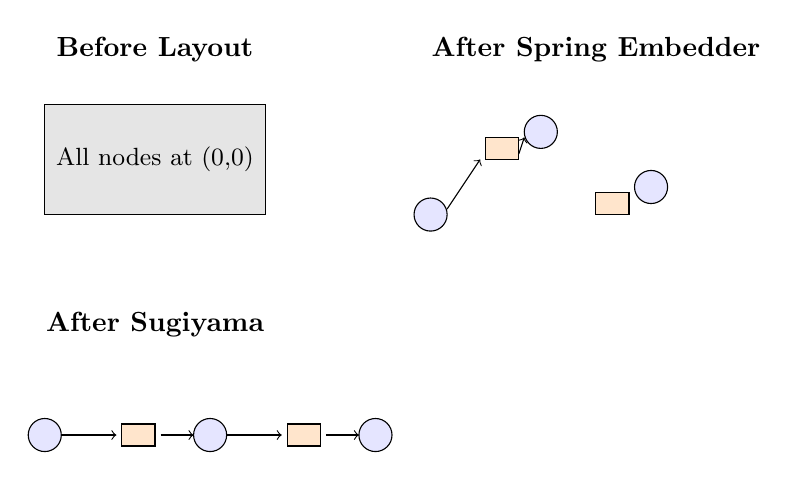
\begin{tikzpicture}[scale=0.7]
        % Before layout
        \node at (-4, 3) {\textbf{Before Layout}};
        \draw[fill=gray!20] (-6, 0) rectangle (-2, 2);
        \node at (-4, 1) {\small All nodes at (0,0)};
        
        % After Spring Embedder
        \node at (4, 3) {\textbf{After Spring Embedder}};
        \draw[fill=blue!10] (1, 0) circle (0.3);
        \draw[fill=blue!10] (3, 1.5) circle (0.3);
        \draw[fill=blue!10] (5, 0.5) circle (0.3);
        \draw[fill=orange!20] (2, 1) rectangle (2.6, 1.4);
        \draw[fill=orange!20] (4, 0) rectangle (4.6, 0.4);
        \draw[->] (1.3, 0.1) -- (1.9, 1);
        \draw[->] (2.6, 1.1) -- (2.7, 1.4);
        
        % After Sugiyama
        \node at (-4, -2) {\textbf{After Sugiyama}};
        \draw[fill=blue!10] (-6, -4) circle (0.3);
        \draw[fill=orange!20] (-4.6, -4.2) rectangle (-4, -3.8);
        \draw[fill=blue!10] (-3, -4) circle (0.3);
        \draw[fill=orange!20] (-1.6, -4.2) rectangle (-1, -3.8);
        \draw[fill=blue!10] (0, -4) circle (0.3);
        \draw[->] (-5.7, -4) -- (-4.7, -4);
        \draw[->] (-3.9, -4) -- (-3.3, -4);
        \draw[->] (-2.7, -4) -- (-1.7, -4);
        \draw[->] (-0.9, -4) -- (-0.3, -4);
    \end{tikzpicture}
    \caption{Layout algorithm results comparison}
    \label{fig:layout-comparison}
\end{figure}

\section{When to Use Which Algorithm}
\label{sec:layout-guidance}

\begin{itemize}
    \item \textbf{Spring Embedder}: 
    \begin{itemize}
        \item Petri nets with many cycles
        \item Organic, symmetric patterns
        \item When hierarchy is not important
    \end{itemize}
    
    \item \textbf{Sugiyama}: 
    \begin{itemize}
        \item Sequential, workflow-like processes
        \item When you want left-to-right or top-to-bottom flow
        \item PNML imports without layout data (default)
    \end{itemize}
\end{itemize}

\section{Summary}
\label{sec:layout-summary}

Layout algorithms transform cluttered diagrams into readable visualizations:

\begin{itemize}
    \item \textbf{Spring Embedder}: Physics-based, produces organic layouts
    \item \textbf{Sugiyama}: Four-phase hierarchical algorithm
    \begin{enumerate}
        \item Cycle removal (DFS-based)
        \item Layer assignment (longest path)
        \item Vertex ordering (barycenter method)
        \item Coordinate assignment
    \end{enumerate}
    \item Both algorithms modify the \texttt{position} property of nodes directly
    \item \texttt{triggerDataChanged(true)} notifies UI to redraw and fit content
\end{itemize}

The next chapter covers the \textbf{Planning Service}, which enables communication with the backend for simulation and analysis.
